% Define custom colors
\definecolor{lightgreen}{rgb}{0.6, 1.0, 0.6}
\definecolor{darkgreen}{rgb}{0.0, 0.5, 0.0}

Since this work is a full dissertation, and now only what is being presented in this part of the report, a work plan has been developed with a timeline for the completion of the work. This timeline start in the $1^{st}$ of January and ends in the $31^{st}$ of October, since this is the deadline for the submission of the dissertation. The work plan in presented in \ref{tab:Work Plan: work plan}. We can see that witting the thesis from the beginning is a priority since this ensures better results and a higher level of coherence in between all the chapter and topics.

\begin{table}[!ht]
    \centering
    \resizebox{0.8\textwidth}{!}{%
        \begin{tabular}{lllllllllll}
        \hline
            \textbf{Tasks} & \textbf{Jan} & \textbf{Feb} & \textbf{Mar} & \textbf{Apr} & \textbf{May} & \textbf{Jun} & \textbf{Jul } & \textbf{Aug} & \textbf{Sep} & \textbf{Oct} \\ \hline
            \textbf{Trajectory Generation} & \cellcolor{darkgreen} & \cellcolor{lightgreen} & ~ & ~ & ~ & ~ & ~ & ~ & ~ & ~ \\ 
            \textbf{Trajectory Optimization} & \cellcolor{lightgreen} & \cellcolor{darkgreen} & \cellcolor{lightgreen} & ~ & ~ & ~ & ~ & ~ & ~ & ~ \\ 
            \textbf{Single Robot Controller} & ~ & \cellcolor{lightgreen} & \cellcolor{darkgreen} & \cellcolor{lightgreen} & ~ & ~ & ~ & ~ & ~ & ~ \\ 
            \textbf{Consensus between system} & ~ & \cellcolor{lightgreen} & \cellcolor{lightgreen} & \cellcolor{darkgreen} & \cellcolor{darkgreen} & \cellcolor{lightgreen} & ~ & ~ & ~ & ~ \\ 
            \textbf{Simulation Study} & ~ & ~ & \cellcolor{lightgreen} & \cellcolor{lightgreen} & \cellcolor{darkgreen} & \cellcolor{darkgreen} & \cellcolor{lightgreen} & ~ & ~ & ~ \\ 
            \textbf{Real world data} & ~ & ~ & ~ &  \cellcolor{lightgreen} & \cellcolor{lightgreen} &\cellcolor{darkgreen} & \cellcolor{darkgreen} & \cellcolor{lightgreen} & ~ & ~ \\ 
            \textbf{Data analysis} & ~ & ~ & ~ & ~ & ~ & \cellcolor{lightgreen} & \cellcolor{darkgreen} & \cellcolor{darkgreen} & \cellcolor{lightgreen} & \cellcolor{lightgreen}\\ 
            \textbf{Dissertation writting} & \cellcolor{lightgreen} & \cellcolor{lightgreen} & \cellcolor{lightgreen} & \cellcolor{lightgreen} & \cellcolor{lightgreen} & \cellcolor{lightgreen} & \cellcolor{lightgreen} & \cellcolor{darkgreen} & \cellcolor{darkgreen} & \cellcolor{darkgreen} \\ \hline
        \end{tabular}
    }
    \caption{Work plan for this dissertation project.}
    \label{tab:Work Plan: work plan}
\end{table}

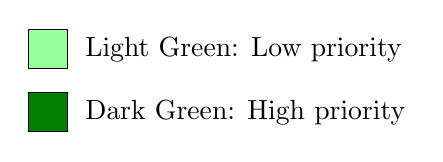
\begin{tikzpicture}
    % Light Green square
    \draw[fill=lightgreen] (0,0) rectangle (0.5,0.5);
    \node[anchor=west] at (0.6,0.25) {Light Green: Low priority};

    % Dark Green square
    \draw[fill=darkgreen] (0,-0.8) rectangle (0.5,-0.3);
    \node[anchor=west] at (0.6,-0.55) {Dark Green: High priority};
\end{tikzpicture}



% Define custom colors
